\section{Introduction and Fundamentals}
\frame{\tableofcontents[currentsection]}
	\subsection{Introduction}
	\begin{frame}
		\frametitle{Introduction}
		kurzes blabla
	\end{frame}
	\begin{frame}
		\frametitle{Flow Properties}
		compressible flow \\
		ideal gas mit gamma
		Ma = def , 0.2
		Re, Pr	
	\end{frame}
	\begin{frame}
		\frametitle{Compressible Navier-Stokes Equation}
		2d\\
		conserved flow variables density, momentum, energy\\
		dimensionless variables\\
		gleichung, aufgeteilt in temporal derivative, convective fluxes, viscous fluxes\\
	\end{frame}
	\subsection{The Runge-Kutta Discontinuous Galerkin Method}
	\begin{frame}
		\frametitle{The Discontinuous Galerkin Space Discretisation}
		\begin{figure}
			\centering
			\subfloat[First order FEM \label{fig:a}]{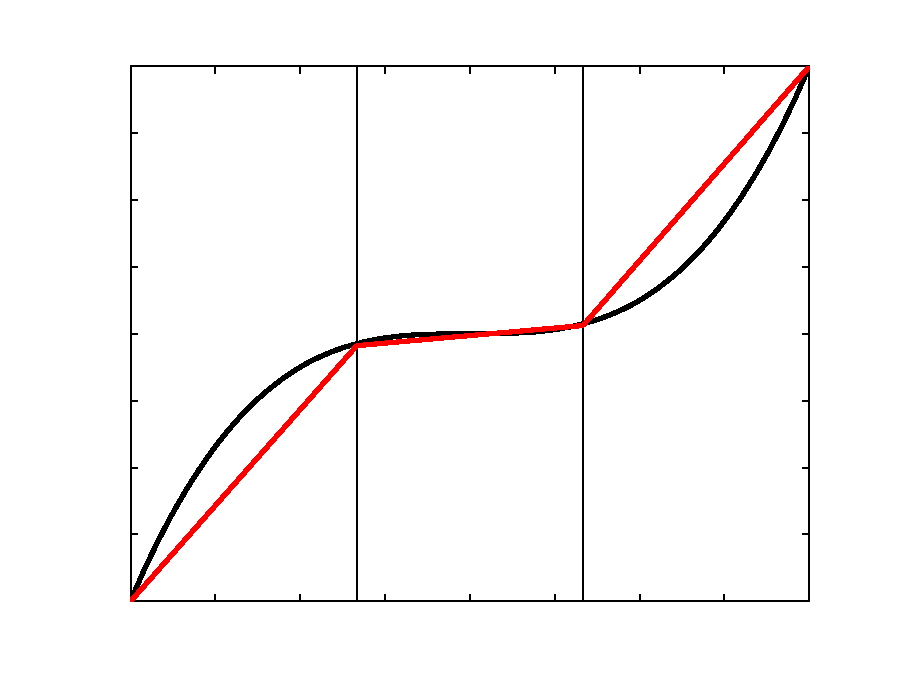
\includegraphics[width=0.28\textwidth]{img/fem.eps}}
			\subfloat[Zeroth order DG (FVM)\label{fig:b}]{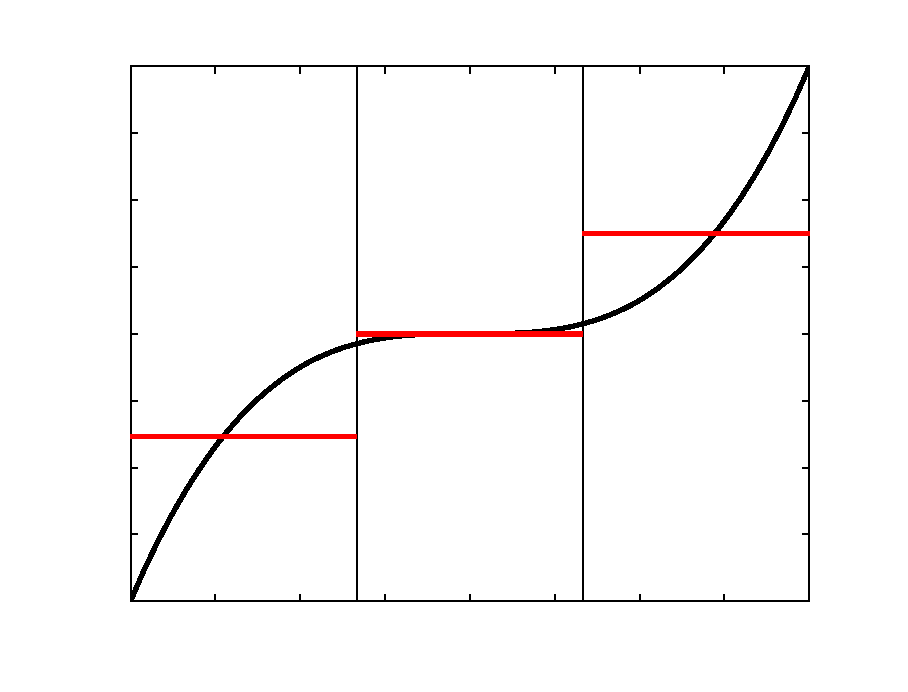
\includegraphics[width=0.28\textwidth]{img/fvm.eps}}
			\subfloat[First order DG \label{fig:c}]{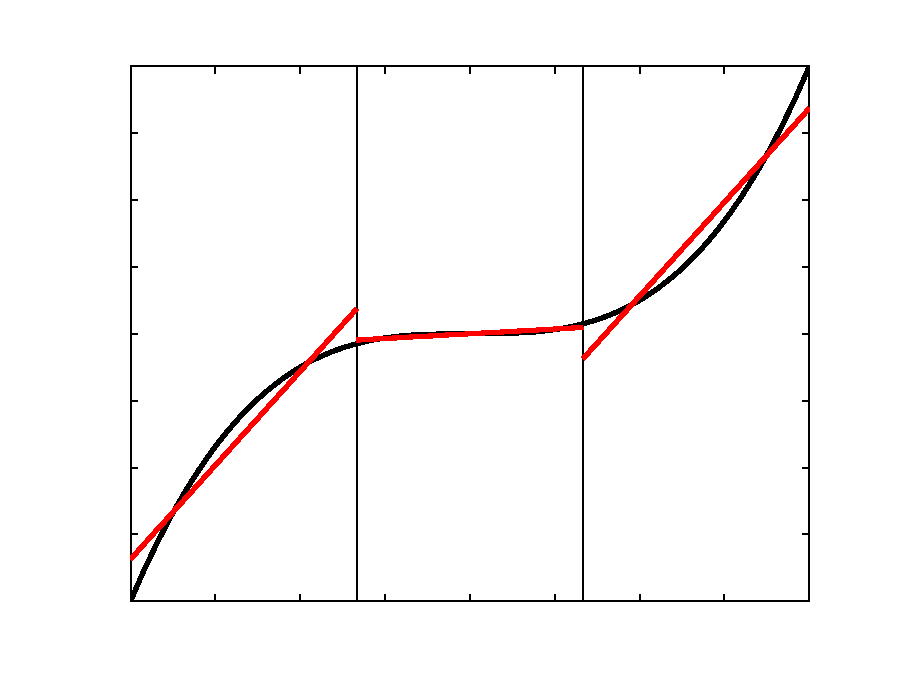
\includegraphics[width=0.28\textwidth]{img/dg.eps}}
			\caption{Comparison of FEM, FVM and DG}
			\label{fig:1}
		\end{figure}

		DG space discretisation Vorgehen, Bildchen, fluxes
	\end{frame}
	\begin{frame}
		\frametitle{The Runge-Kutta Time Discretisation }
		RK time discretisation Endformel, Tabelle, cfl criterion
	\end{frame}
	\subsection{The Immersed Boundary Method}
	\begin{frame}
		\frametitle{The Immersed Boundary Method}
		regions mit Bild, Aufteilung Integrale
		mass matrix
		rk time discretisation formel
		cell agglomeration
	\end{frame}